\documentclass[a4paper,twoside]{style/article}

\usepackage{epsfig}
\usepackage{subfigure}
\usepackage{calc}
\usepackage{amssymb}
\usepackage{amstext}
\usepackage{amsmath}
\usepackage{amsthm}
\usepackage{multicol}
\usepackage{pslatex}
\usepackage{apalike}
\usepackage{style/SCITEPRESS}
\usepackage[small]{caption}

\subfigtopskip=0pt
\subfigcapskip=0pt
\subfigbottomskip=0pt

% My Packages and Commands ---
\usepackage[normalem]{ulem}
\usepackage{xcolor}
\newcommand{\rem}[1]{\textcolor{red}{\sout{#1}}}
\newcommand{\add}[1]{\textcolor{blue}{\uline{#1}}}
\newcommand{\com}[1]{\textcolor{orange}{\uline{#1}}}
% /My Packages and Commands --

\begin{document}

\title{Insight Into Lumbar Back Pain  \subtitle{What the Lumbar Spine Tells About Your Life} }

\author{\authorname{Paul Klemm\sup{1}, Sylvia Glaßer\sup{1}, Kai Lawonn\sup{1} Henry Völzke\sup{2} and Bernhard Preim\sup{1}}
\affiliation{\sup{1}Department of Simulation and Graphics, University of Magdeburg}
\affiliation{\sup{2}Greifswald}
% TODO: Mailaddy nachtragen
\email{\{paul, sylvia\}@isg.cs.uni-magdeburg.de, voelzke@anderAddy}
}

% TODO: The paper must have at least one keyword. The text must be set to 9-point font size and without the use of bold or italic font style. For more than one keyword, please use a comma as a separator. Keywords must be titlecased.
\keywords{My Keywords in Title Case}

\abstract{The abstract should summarize the contents of the paper and should contain at least 70 and at most 200 words. The text must be set to 9-point font size.}

\onecolumn \maketitle \normalsize \vfill

\section{\uppercase{Introduction}}
\label{sec:Introduction}
Epidemiology is the study of causation of diseases.
%%
Large population studies, such as the Study of Health in Pomerania (SHIP) \ref{SHIP} gather as much information as possible about participants to be assessed towards different diseases.
%%
These information are used to determine risk factors for diseases, helping people to make their lifestyle healthier or helping in diagnosing a disease.
%%
Epidemiological research is strongly hypothesis driven.
%
Observations made by clinicians are translated into hypothesis, which are then statistically evaluated using data variables from epidemiological studies.

Modern cohort studies often comprise medical image data.
%%
These data are hard to analyze, since segmentation algorithms are not generally available and need to be custom-made for each body structure.
%%
Segmentation data it is usually analyzed by abstracting it into key figures, making it statistically comparable to non-image variables and retrieve correlations.
%%

Back pain is one of the most frequent diseases in the western civilization.
%%

Our goal is to combine data mining algorithm with data visualization to provide insight into the quality of image derived data to analyze if it acts as a risk factor for a disease.
%\com{Combine Data Mining Algo}

More than 5 variables are rarely analyzed simultaneously.
%%
%The variables analyzed simultaneously is limited to 
Our contributions are:
\begin{itemize}
	\item Analyzing back pain using image-derived variables of 2,240 subjects.
	\item Assessing the suitability of lumbar spine shape for diagnosing back pain
	\item Analyzing correlations between between image-based and socio-demographic as well as medical parameters.
\end{itemize}

\section{\uppercase{Epidemiological Background}}
 \ref{VIS14}
\label{sec:EpidemiologicalBackground}
\noindent \com{Background. Epidemiological Workflow, focus on statistical resilience, image data hard to analyze due to the large amount of subjects, poor image quality and lack of methods}.
\subsection{Back Pain}
\com{Back pain one of the most common diseases in the western civilization; hard to analyze; Epidemiologists interested in the \emph{healthy} aging process}.

\section{\uppercase{Related Work}}
\label{sec:RelatedWork}
\noindent \com{Our own work (VIS, VMV, BVM). Sylvias paper with reference to the methods. \textbf{More information necessary here!}}

\section{\uppercase{Materials and Method}}
\begin{figure}[!h]
  %\vspace{-0.2cm}
  \centering
  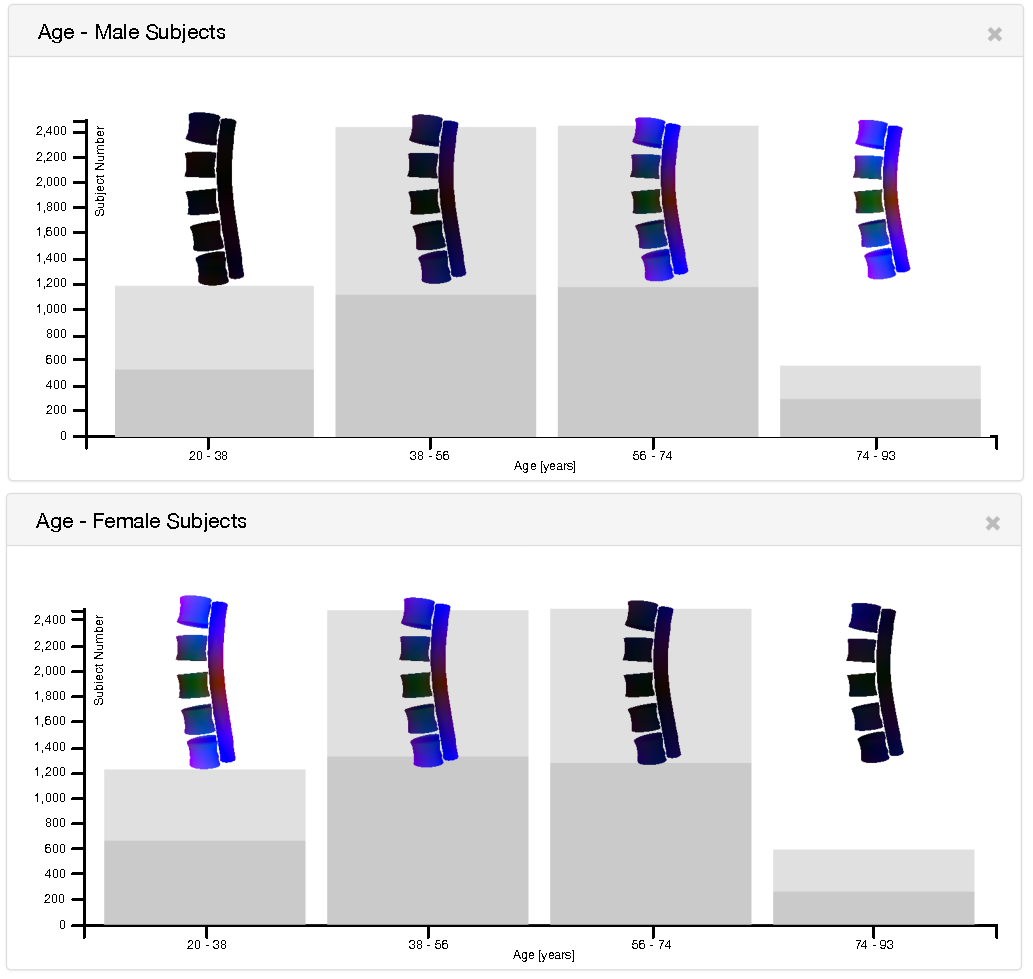
\includegraphics[width=0.5\textwidth]{figures/age-gender}
  \caption{Age-Gender}
  \label{fig:example1}
 \end{figure}
\label{sec:MaterialsAndMethod}

\subsection{The Lumbar Spine Data Set}
Our data set compiled to analyze lumbar back pain comprises of 6,753 subjects from two cohorts (4,420 from \texttt{SHIP-Trend-0} and 2,333 from \texttt{SHIP-2}).
%%

%%

\subsubsection{Image Data}
\com{From VIS'14 Paper}
The lumbar spine was detected in the image data using a hierarchical finite element method by Rak et al. [32]. This semiautomatic method requires the user to initialize the tetrahedron-based finite element models (FEM) with a click on the L3 vertebra. Two user-defined landmarks on the top and bottom of the L3 vertebra describe an initial model height estimation. The model uses a weighted sum of T1and T2-weighted MR images to detect the lumbar spine shape. Once registered, it captures information about the shape of the lumbar spine canal as well as the position of the L1-L5 vertebrae [21]. Due to incorrect initialization, strongly deformed spines, contrast differences and artifacts, the model was not able to detect lumbar spines for all subjects. We obtained and worked with 2,540 tetrahedron models of the lumbar spine. For clustering, we extracted the centerline of the lumbar spine canal, which captures information about lordosis and scoliosis (the medical terms for spine curvature) [21].

\subsubsection{Non-Image Data}
\com{Analysis Using Heterogeneous Correlation}
The variables range from somatometric variables describing body measures to medical examinations, such as laboratory tests as well as lifestyle factors as sport activity or nutrition.

\subsection{Creating a Decision Tree using C5.0}
\com{C4.5 Algorithm for creating decision trees; }

\subsection{Parameter Assessment}


\section{\uppercase{Experiments}}
\label{sec:Experiments}
\subsection{Results}
\com{We can discriminate back pain using non-image data, but not with image-derived parameter}

\section{\uppercase{Experiments}}
\label{sec:Experiments}

\section{\uppercase{Conclusion}}
\label{sec:Conclusion}

\section*{\uppercase{Acknowledgements}}

\noindent SHIP is part of the Community Medicine Research net of the University of Greifswald, Germany, which is funded by the Federal Ministry of Education and Research (grant no. 03ZIK012), the Ministry of Cultural Affairs as well as the Social Ministry of the Federal State of Mecklenburg-West Pomerania. Whole-body MR imaging was supported by a joint grant from Siemens Healthcare, Erlangen, Germany and the Federal State of Mecklenburg-Vorpommern. The University of Greifswald is a member of the ‘Centre of Knowledge Interchange’ program of the Siemens AG. This work was supported by the DFG Priority Program 1335: Scalable Visual Analytics.


\vfill
\bibliographystyle{style/apalike}
{\small
\bibliography{bibliography}}


\section*{\uppercase{Appendix}}

\noindent If any, the appendix should appear directly after the
references without numbering, and not on a new page. To do so please use the following command:
\textit{$\backslash$section*\{APPENDIX\}}

\vfill
\end{document}

